\label{sec:discussion}

Table~\ref{tab:main-results} and Figure~\ref{fig:param-efficiency} together summarise the experiments. The parameter efficiency scatter is the single visual that captures our thesis.

\begin{table}[H]
\centering
\small
\begin{tabular}{lccc r}
\toprule
Method & Test Acc (\%) & MPC Acc (\%) & Top-5 (\%) & Trainable params \\
\midrule
\textbf{VPT-Deep}           & \textbf{91.64} & \textbf{92.83} & \textbf{97.93} & \textbf{170{,}598} \\
Frozen ResNet18             & 88.52 & 90.82 & --- & 10{,}545{,}766 \\
Label smoothing             & 87.27 & 89.40 & --- & 11{,}228{,}838 \\
ResNet50                    & 85.93 & 88.07 & --- & 23{,}717{,}030 \\
VPT-Shallow                 & 84.13 & 85.70 & 95.43 & 86{,}118 \\
Baseline                    & 84.42 & 86.11 & --- & 11{,}228{,}838 \\
Deformable                  & 81.33 & 83.46 & --- & 11{,}415{,}534 \\
MixUp                       & 80.52 & 83.50 & --- & 11{,}228{,}838 \\
Hybrid (ours)               & 78.73 & 81.34 & --- & 11{,}353{,}290 \\
Dilated                     & 75.95 & 78.53 & --- & 11{,}228{,}838 \\
Depthwise                   & 57.03 & 59.71 & --- & 1{,}623{,}270 \\
\bottomrule
\end{tabular}
\caption{Test-set results for every model we trained, sorted by mean per-class accuracy.}
\label{tab:main-results}
\end{table}

\begin{figure}[H]
\centering
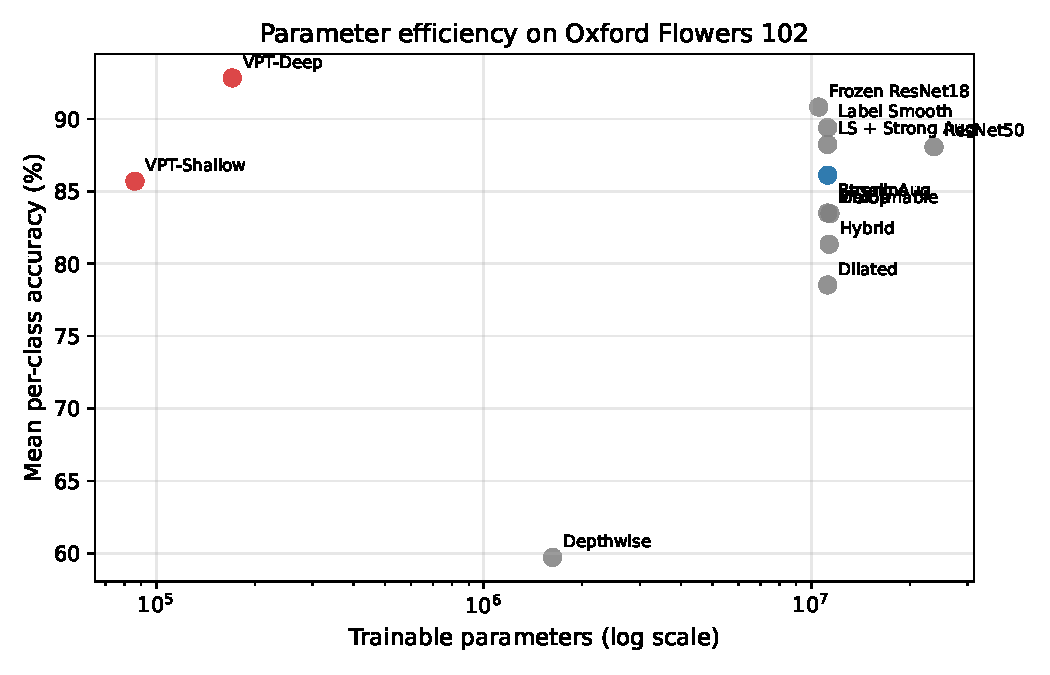
\includegraphics[width=0.8\textwidth]{figures/parameter-efficiency.pdf}
\caption{Mean per-class accuracy versus trainable parameter count. VPT variants sit in the top-left corner (best accuracy at smallest parameter count). CNN variants occupy the middle-right region.}
\label{fig:param-efficiency}
\end{figure}

\textbf{What worked.} VPT-Deep outperformed every CNN configuration we trained. Freezing the first two ResNet18 layers was the most useful CNN intervention. Label smoothing gave a small but cheap improvement. Scaling to ResNet50 produced a modest gain that did not justify its extra cost.

\textbf{What did not work, and why.} Four findings went against common defaults:

\emph{Dilated, deformable, and hybrid convolutions hurt.} All four convolutional modifications we tested dropped MPC accuracy below the baseline, despite being well-motivated on paper. The shared cause is the mismatch between the pre-trained weights and the new operator. Dilation spreads the sampling grid across a wider area than the weights were trained for. The deformable offset predictor starts from a zero initialisation and needs more data than 1020 images to learn useful offsets.

\emph{Depthwise-separable convolution collapses.} With the kernel shape changed, pre-trained weights cannot be copied and the model learns from scratch. Fifty epochs of 1020 images are not enough to make this viable.

\emph{MixUp hurts at ten shots per class.} MixUp is a default regularizer in most vision pipelines, but under extreme data scarcity it damages performance. With 102 classes and 10 examples each, most mixed pairs cross unrelated species, and the resulting soft labels carry little class-discriminative signal.

\emph{Strong augmentation alone does not help.} RandomResizedCrop and ColorJitter together produced the same MPC accuracy as the baseline, suggesting Flowers 102 already tolerates mild geometric variation and that the true bottleneck is overfitting to class identity, not to pose.

\textbf{Why VPT-Deep wins.} Two forces compound. First, its parameter budget is 60 to 140 times smaller than the CNN alternatives, which limits overfitting. Second, it never disturbs the pre-trained backbone. The learnable prompts act as task-specific queries that reshape the input distribution seen by the frozen Transformer layers, without asking those layers to change what they computed on ImageNet-21k. Few-shot results make the second point concrete: the gap between VPT-Deep and the best CNN widens as training data shrinks, because the CNN has more parameters to spoil and fewer examples to constrain them.

\textbf{Comparison to prior work.} \citet{nilsback2008} reported 72.8\% accuracy with hand-engineered features and a multiple-kernel SVM. Our VPT-Deep result (91.64\% test accuracy) is consistent with the general Transformer-based numbers from recent work, though direct comparison is difficult because many recent papers use larger backbones (ViT-L/14), additional tricks, or different train/test splits. \citet{jia2022vpt} reported 89.11\% average across five FGVC datasets for VPT-Deep on a ViT-B/16 pre-trained on ImageNet-21k; our 92.83\% MPC on ImageNet-1k pre-trained weights sits above that average.

\textbf{Limitations.} We evaluate a single seed and a single backbone. Variance across seeds is an obvious gap. We also did not implement triplet loss (noted as a future-work suggestion in the project handout) or test-time augmentation, both of which could push the numbers higher. The prompt length ablation (Figure~\ref{fig:prompt-length}) shows that $p=50$ beats our $p=10$ default, so the VPT-Deep results reported in Table~\ref{tab:main-results} are not the best the method can do.
